% 【文書名】無題
% 【著者】片山博文MZ
%%%%%%%%%%%%%%%%%%%%%%%%%%%%%%%%%%%%%%%%%%%%%%%%%%%%%%%%%%%%%%%%%%%%%%%%%%%%%
% LuaLaTeX使用.

\RequirePackage{plautopatch} % pLaTeXのいろいろな不具合を修正する

\documentclass[a4paper,11pt,twocolumn]{ltjsarticle} % 記事の場合
%\documentclass[a4paper,11pt,twocolumn]{ltjsreport} % 報告書の場合

% a4paper, b5paperは、用紙サイズ.
% 文字のサイズは 10pt, 11pt, ... などから選べる.
% twocolumnは二段組の場合に指定する.
% LuaLaTeXでない場合は「\documentclass[dvipdfmx, ...」などと書かないといけない.

%%%%%%%%%%%%%%%%%%%%%%%%%%%%%%%%%%%%%%%%%%%%%%%%%%%%%%%%%%%%%%%%%%%%%%%%%%%%%
% プリアンブル開始

\usepackage{amsmath,amssymb} % AMS数式
\usepackage{amsthm} % 定理環境
\usepackage{graphicx} % 画像を使う
\usepackage{xcolor} % 色を使う
\usepackage{url} % URLを記述するときに使う
\usepackage{hyperref} % ハイパーリンクで参照
\usepackage[margin=18truemm]{geometry} % 余白を18mmにする(印刷用紙を節約)
\usepackage{type1cm} % Computer Modernフォントを使わない

%% ソースコードを埋め込みたい場合(listings.styのインストールが必要)
%\usepackage{listings} % ソースコードを取り込むパッケージ
%\def\lstlistingname{ソースコード}
%\lstset{
%	language=c,
%	breaklines = true,
%	basicstyle=\ttfamily\scriptsize,
%	commentstyle={\textmc},
%	classoffset=1,
%	keywordstyle=\bfseries,
%	showstringspaces=false,
%	frame=tblr,
%	numbers=left,
%	stepnumber=1,
%	numberstyle=\tiny,
%	tabsize=2
%}

\newcommand{\mathref}[1]{(\ref{#1})} % コマンドを定義
\newcommand{\combination}[2]{{}_{#1} \mathrm{C}_{#2}} % コマンドを定義

% 定理、命題など
\newtheorem{thm}{定理}
\newtheorem{lem}[thm]{補題}
\newtheorem{prop}[thm]{命題}
\newtheorem{cor}[thm]{系}
\newtheorem{ass}[thm]{仮定}
\newtheorem{conj}[thm]{予想}
\newtheorem{dfn}[thm]{定義}
\newtheorem{rem}[thm]{注}
\renewcommand{\proofname}{\textbf{証明}}

% プリアンブル終了
%%%%%%%%%%%%%%%%%%%%%%%%%%%%%%%%%%%%%%%%%%%%%%%%%%%%%%%%%%%%%%%%%%%%%%%%%%%%%

\begin{document} % 文書開始

\title{無題}
\author{片山博文MZ\footnote{宮崎市在住のアマチュア数学屋}}
\date{\today}
\maketitle

% \tableofcontents % 目次

\section{はじめに}

この文書は,日本語LuaLaTeXの書き方を示すものである.

\subsection{数式}

次の数式\mathref{eq:trivial}はつまらない.

\begin{equation}
1 = 1 \label{eq:trivial}
\end{equation}

次の数式は面白い.

\begin{equation}
A = \begin{pmatrix}
	a_{11} & \ldots & a_{1n} \\
	\vdots & \ddots & \vdots \\
	a_{m1} & \ldots & a_{mn}
	\end{pmatrix}
\end{equation}

\begin{equation}
\combination{n}{k} = \frac{n!}{k! (n-k)!}
\end{equation}

\subsection{番号付き箇条書き}

\begin{enumerate}
\item 項目1
\item 項目2
\item 項目3
\end{enumerate}

\subsection{番号なし箇条書き}

\begin{itemize}
\item 項目1
\item 項目2
\item 項目3
\end{itemize}

%\subsection{ソースコード}
%
%\lstinputlisting[caption=Hello Worldを表示するプログラム,label=hello]{hello.c}

\subsection{引用その1}

\begin{quote}
ここは引用です.
\end{quote}

\subsection{引用その2}

\begin{quotation}
ここは引用です.
\end{quotation}

\subsection{図と表}

\begin{figure}[b] % 図の開始
\centering % 図を中央揃え
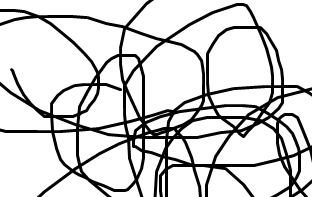
\includegraphics[width=3cm]{images/fig1.png}
\caption{つまらない画像}
\label{fig:fig1}
\end{figure} % 図の終わり

\begin{table}[b] % 表の開始
\centering % 表を中央揃え
\begin{tabular}{|l||r|r|}
品名 & 単価(円) & 個数 \\
\hline
リンゴ & 100 & 5 \\
みかん & 50 & 10
\end{tabular}
\caption{つまらない表}
\label{tab:tab1}
\end{table} % 表の終わり

\subsection{色と太字}

\textcolor{red}{これは赤}です.
\textbf{これは太字}です.

\subsection{参照}

つまらない数式は,\pageref{eq:trivial}ページの式\mathref{eq:trivial}にある.

つまらない表は,\pageref{tab:tab1}ページの表\ref{tab:tab1}にある.

つまらない画像は,\pageref{fig:fig1}ページの図\ref{fig:fig1}にある.

URLは,\url{https://example.com} のように使う.

\section{定理など}

\begin{thm} % 定理
私以外は私ではない.
\end{thm}

\begin{proof} % 証明
自明.
\end{proof}

\section{終わりに}

\cite{bib:mybook}が大変,役に立たなかった.

\begin{thebibliography}{99}
\bibitem{bib:mybook}
	片山博文MZ『つまらない本』つまらない出版社,2025.
\end{thebibliography}

\end{document} % 文書終わり

%%%%%%%%%%%%%%%%%%%%%%%%%%%%%%%%%%%%%%%%%%%%%%%%%%%%%%%%%%%%%%%%%%%%%%%%%%%%%
